% !TeX root = ../../main.tex
\chapter{Requirements}
\label{chap:requirements}

\section{Process Used for Capturing Requirements}

\section{Requirements Specification}

\section{The Problem}
With smart devices being created left right and centre nowadays with very little care towards security, it is going to become more common that houses are being hacked with devices slowly controlling more and more sensitive areas of the home. An example of this would be the August lock, an idea similar to what I am trying to achieve here, however the device has multiple security flaws that were found and outlined at the security conference Defcon. This is far from the first smart home device that was found to have security issues, there have been hundreds of different WiFi Security cameras that connect themselves to the web with little care towards the security of that device which has the capability of letting someone spy on your home. Not to long ago, there was a huge attack that brought down DynDNS, and therefore all the sites that used it which included Twitter, Spotify and Reddit. This attack was using the internet connections of innocent people who happened to have insecure smart home devices in their homes. Millions of smart home devices were involved in the attack as they were hacked due to their inadequate or sometimes non-existent security.
\newline
\newline
I want to create a product unlike these other smart home devices, one that is secure enough that I would be happy to put it in my own home. At the end of the day, a camera being infected doesn't matter so much, but a system that unlocks your house needs to be bulletproof on the security front. Looking at the implementation of the August lock, it just isn't something that I would be willing to use to secure my house, yet thousands, maybe more unknowing customers have purchased the august lock and use it to secure their homes every day. I want to create something that is easy to use, and secure, something that most companies seem to have trouble with nowadays.

\section{Aim of the Project - Technical}
The project objective is to create a smart lock system that would be able to automate the unlocking and locking of a house's front door. The system will be comprised of multiple Raspberry Pi's with sensors connected to them to retrieve data from a variety of sources to determine whether the door should be locked or unlocked. The system will use RESTful APIs so that it can be easily extended to more devices in the future, and will ensure that all communication between devices is done so in a fully encrypted and secure manner. An example of some authentication methods that the system may use would be fingerprint, RFID/NFC, Facial Recognition, etc.
\newline
\newline
Security is key as this will be securing a home. It is imperative that all communication is done securely, and that the system is certain that the user is who they say they are before they let them into the house. I will be conducting research into the best and most accessible security methods that could be used for this project for the initial implementation and demonstration. The idea however, is that the system will be built in such a way that anyone could create a device for this system using the RESTful APIs that will be available from the core control centre in the house.

\section{Aim of the Project - For the User}
So security is all well and good, but the product must still be easy to use for the user. At the end of the day, a lot of users don't care about how secure a product is, and will trust that the company has put in the correct security measures. This reason alone is why there are so many unsecured smart devices out in the wild as your average person doesn't have the technical knowledge to ensure that the product is secure. The companies that make these products know this and so don't actually implement robust security, something that, in my opinion, should be regulated more closely. This product should make the users lives easier whilst still maintaining the security of any normal key based locking system.
\newline
\newline
A simple run down of what I would want from this lock for the user would be the following. They walk up to their home after having setup their system, and all they need to do to get in is tap their phone on the NFC pad in order to unlock the door, and have it lock itself again after they have entered the house, probably on a timer of some sorts. If the door fails to lock for any reason, the user should be notified (another issue with the august lock, if it fails to lock, it simply reports the door as locked, even if it isn't).

\cite{Lackner2013}

\section{Project Objectives}
\begin{itemize}
	\item Design a Database Schema that can be used to store all the users data and settings efficiently
	\item Develop a core application for the house that will control the main system functions
	\item Develop a REST API for the core application that other systems (i.e. authentication systems) can talk to
	\item Implement a minimum of two authentication methods that can be used to unlock the door
	\item Develop a server system that can be used for the core to sync with and for the user to communicate with the system when outside of the home
	\item Develop a minimal Android application that the user can use to setup and manage their system
	\item Ensure that the security of the product is solid and that all communication is secured with TLS 1.2
\end{itemize}

\section{Risk Management}
For a project such as this, there is obviously a large amount of risk involved if for some reason the system isn't secured correctly. My plan is to limit these risks as much as possible by ensuring that all communication is using enforced TLS 1.2 as well as not running the system on an actual door until I have a working system that I have run penetration testing on. Replay attacks were something that I had to consider, but these are averted by using TLS 1.2, as it has protection against that built in using the MAC secret and the sequence number. When running this system on a real door, there will be much larger risk involved as it is obviously securing a real house, however as long as all the proper testing is done before it gets installed on a real door, then that should eliminate the risk involved. Obviously, if this gets installed on any door, then it will be in my own house, so I will ensure that the system is functioning properly before installation and any updates are fully tested before being installed on the live system.

\newpage
\section{Project Plan}
\begin{center}
	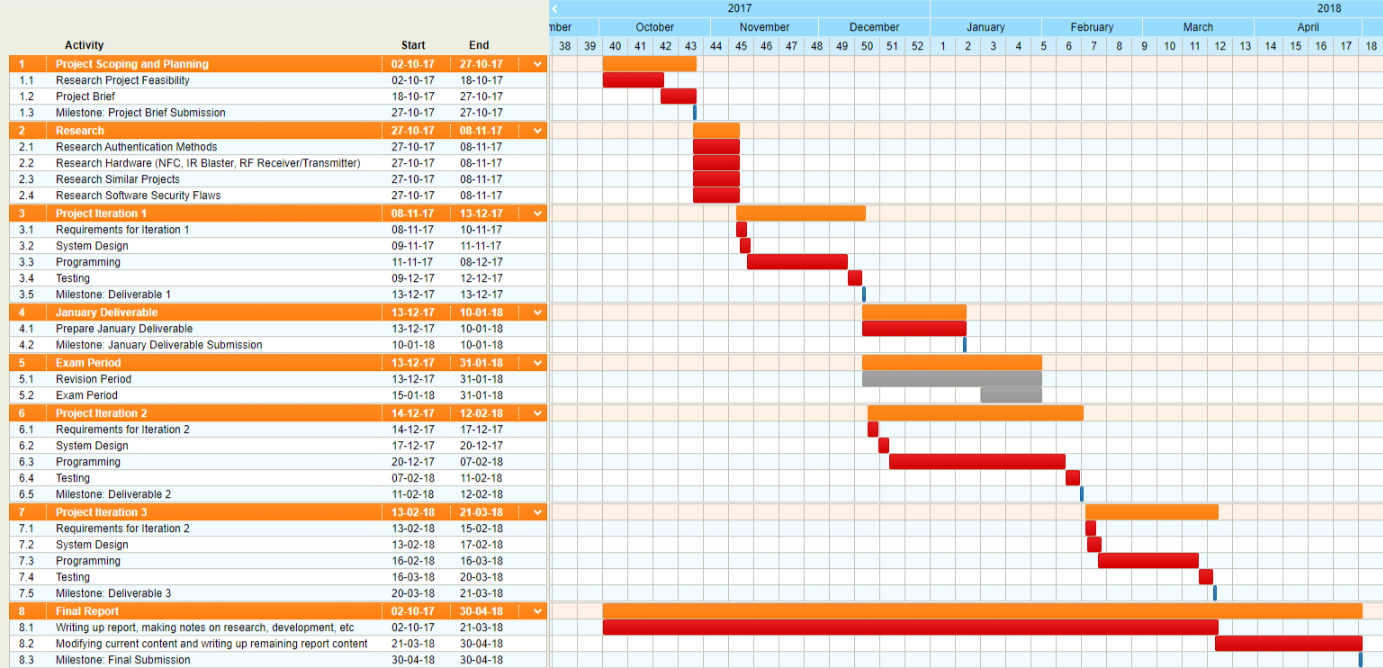
\includegraphics[angle=90,width=\textwidth,height=\textheight,keepaspectratio]{Graphics/FYP-Project-Plan}
\end{center}

\newpage
\section{Block Diagram}
\begin{center}
	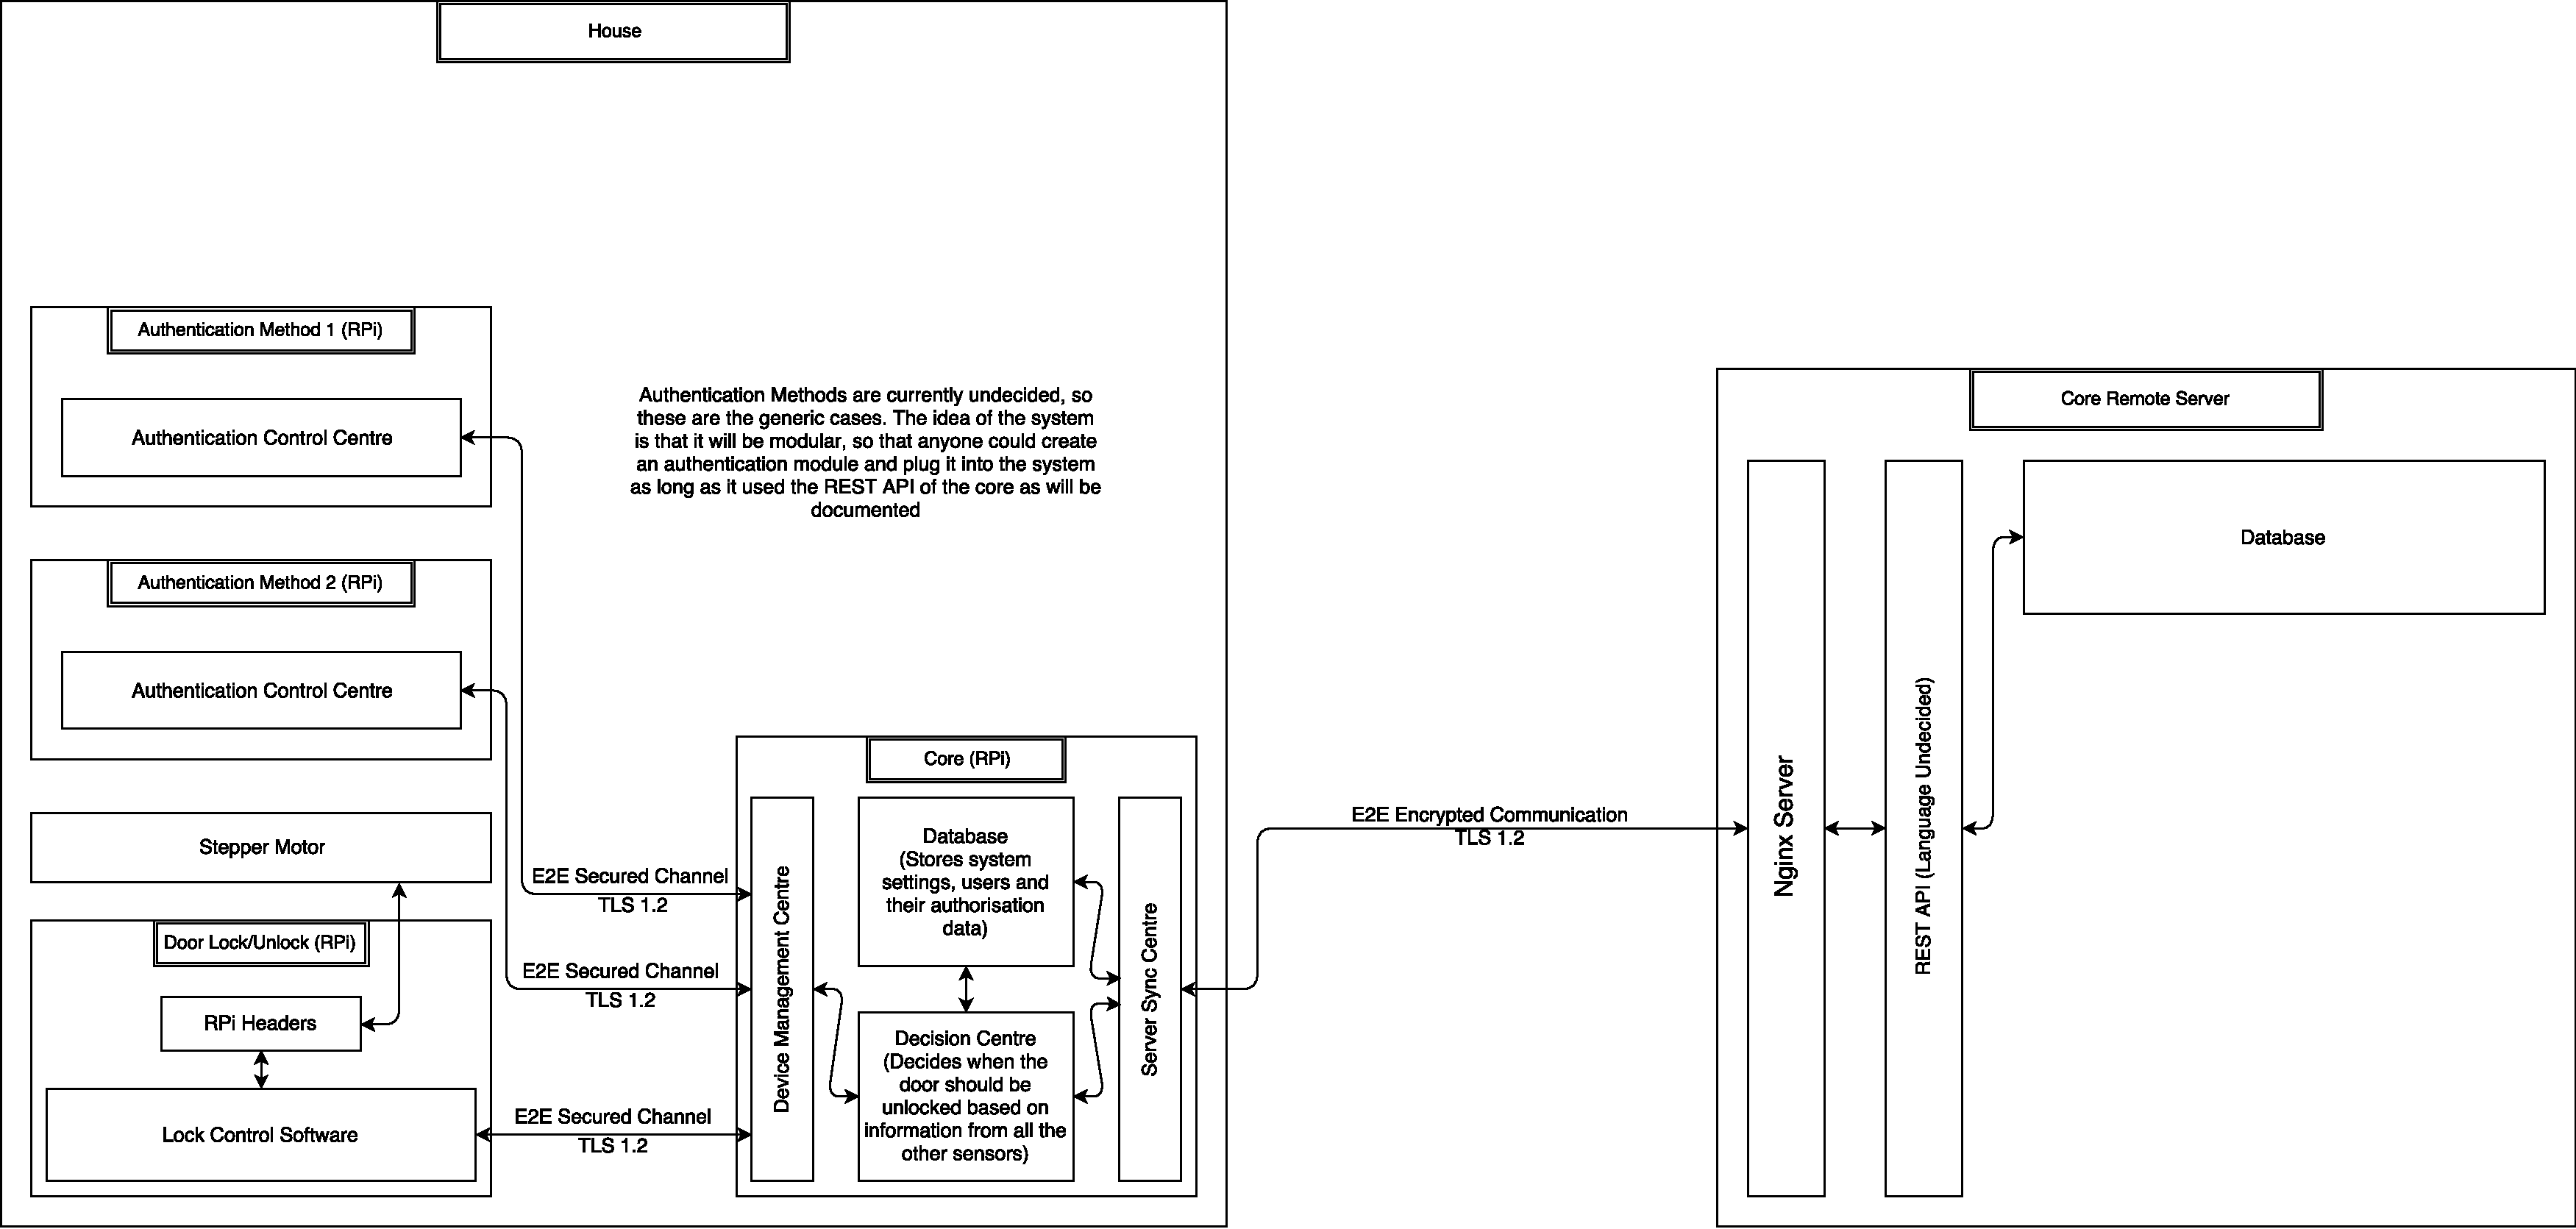
\includegraphics[angle=90,width=\textwidth,height=\textheight,keepaspectratio]{Graphics/FYP-Block-Diagram}
\end{center}

\newpage
\section{Sequence Diagrams}
\subsection{Initial Core Raspberry Pi Setup}
\begin{center}
	\includegraphics[width=\textwidth,height=\textheight,keepaspectratio]{"Graphics/Initial Core RPi Setup"}
\end{center}

\newpage
\subsection{New Device Pairing to Existing Network}
\begin{center}
	\includegraphics[width=\textwidth,height=\textheight,keepaspectratio]{"Graphics/New Device Pairing to Network"}
\end{center}

\newpage
\section{Software Development Project}

\subsection{Requirements Analysis and Specification}

\subsection{Design}
In this section I will describe certain aspects of the project where I had to make decisions as to how they could be implemented best. In each section I will give a high level description of each method followed by which method I decided to go with and why.

\subsubsection{Initiate Connection from Another Device to Core Raspberry Pi}
This is a difficult issue to get around as finding a specific device on the network is not trivial, especially if the network is particularly large. There are various different ways I could solve this which are described below.

\paragraph{Method 1 - IP Broadcasting} One option is to use IP Broadcasting, where the core uses the networks broadcast range to send data to all the other devices on the network. This would work, but I'm unsure of the reliability of this method and broadcasting the IP of the core to the entire network doesn't seem like something I would want to do. It would likely be fine on a home network, however if it was on a much larger network in a business, this method may not work at all as they could block broadcasting on their switches entirely, or if multiple cores are running on the network it could become quite congested with the number of devices trying to announce themselves to other devices.

\paragraph{Method 2 - Bluetooth Sync Device to Core} This would use the Bluetooth on both devices to contact each other and find out the IP of the core on the network. The device would then use this IP to establish a connection to the core. This method has a few issues, namely the security of communicating over Bluetooth as it doesn't have the same kind of security as Wi-Fi. The other issue is that this means the two devices must be within Bluetooth range, which is much shorter than Wi-Fi range and can't be easily extended, unlike Wi-Fi range which has highly available and cheap range extenders.

\paragraph{Method 3 - Contact the remote server to get the Core IP} For this to work, the Core would have to announce its IP to the remote server whenever it changed. This would be very simple as the Core will already have a connection established to the remote server. The device that is trying to connect to the Core would then simply have to contact the remote server and request the IP of the Core on the local network, and then establish a connection with it. This is the easiest method to secure as it gives one point of contact to retrieve this information, and eliminates the need for any kind of discovery. This also allows devices to be as far away from each other as required if they are on the same network.

\paragraph{Decision}
\info{Write this section}

\subsubsection{Initiate Connection to Core Raspberry Pi for Initial Setup}

\paragraph{Method 1 – Connect using 4-digit code through the remote server}
The first issue here is that using a code means that you don’t have to be within proximity of the device to attach to it as it goes through the remote server to establish the link. There are some potential ways that attackers could guess or work out the code and then connect to it themselves, or find some way to force the remote server to override the owner of that Core. The initial setup should be handled on the Core itself, and the phone should not contact the remote server regarding this, the Core should contact the remote server to establish that a link has been created.

\paragraph{Method 2 – Connect using Bluetooth sync between the Core and users phone}
This method requires that the user is close to the Core to establish a link with it as they must be within Bluetooth range and push a physical button on the device to start the pairing process. If the device is already paired to an account, then it will either need to be confirmed by the current account that they want to pair to a new account or they will need to wait for a timeout to expire before the pairing can be done (unless it is cancelled from the current owners account). Within the app, they will need to select the option to connect to a new Core, and then select the Core they want to pair with from the list. The phone will then establish a Bluetooth connection with the Core, the Core will generate a private key to identify itself, and will upload the public key to the remote server for validation when communicating with it. This will bind the Core to the account the user was logged into and they will then be able to add new devices and users to the Core, as well as modify the settings for the Core, all from the app.

\paragraph{Method 3 – Connect to Wi-Fi network broadcasted by the Core on users phone}
This method requires that the used must be close to the Core to push the physical button on the device to create the Wi-Fi network to start the setup of the device. All other steps are the same as Method 2, however this method has the benefit of not requiring every device to have Bluetooth as well as Wi-Fi, lowering the physical size, cost and power required to run each device. Wi-Fi can also be more easily secured than Bluetooth, and I will carry out testing to see if I can lower the power of the Wi-Fi adapter when in access point mode to lower the range of the network, so the user must be close to the device when performing the initial setup. I will be using this method instead of the method 2 for the reasons mentioned prior.

\paragraph{Decision}
\info{Write this section}

\subsubsection{Initiate Connection from New Device to Core Raspberry Pi for Setup}

\paragraph{Method 1 – Bluetooth pairing between Device and Core}
This method would work, but could introduce difficulties for the user as it requires the two devices to be close to each other as they must be within Bluetooth range. It would also require the core to store the Wi-Fi password in a readable form to give it to new devices that will also need it. This is not something that I want to do as that means if someone can access the device then they can access the Wi-Fi password and therefore the entire network.

\paragraph{Method 2 – Bluetooth pairing between device and users phone}
This method will work in the same way as the initial setup of the core. The User will press a pairing button on the device itself, then go to an add device page on their phone (only available for people who are already admins of a Core). On this page they will see any devices that are in pairing mode that they can add to their network. Once they have added the device, the app will request they connect it to the same Wi-Fi network as the Core, and request the password for the network. The device will then have successfully been added to the door unlocking system, will exit syncing mode, and will then communicate with the Core directly. The user will see the device in their list of devices on their door unlocking system, and will be able to change any settings it has.

\paragraph{Method 3 – Wi-Fi pairing between the device and users phone}
\improvement{This section should be re-written and improved upon}This method will work in the same way as method 2, however it will use Wi-Fi instead of Bluetooth for the setup, for the same reasons mentioned in Method 3 of the initial setup of the core section.

\paragraph{Decision}
\info{Write this section}